\documentclass{beamer}

\usepackage{beamerthemetree}
\usepackage{tabularx}
\usetheme{Boadilla} 
\usecolortheme{whale}

\usepackage{graphicx}
\usepackage[absolute,overlay]{textpos}
\usepackage{hyperref}

\usepackage{verbatim}

\usepackage{color}
\definecolor{nasa_blue}{rgb}{0.14117,0.36863,0.66666}
\definecolor{openmdao_red}{rgb}{0.545,0.0,0.0}
\definecolor{forestgreen}{rgb}{0.18,0.52,0.18}
%\definecolor{alt_background}{rgb}{.506,.224,.725} %purple
%\definecolor{alt_background}{rgb}{.141,.165,.196} %dark blue/gray
\definecolor{alt_background}{rgb}{.376,.396,.427} %light blue/gray

\usepackage[normalem]{ulem}

\usepackage{geometry}
\usepackage{amsfonts}
\usepackage{amsmath}
\usepackage{amssymb}
\usepackage{tikz}
\usepackage{booktabs}
\usepackage{anyfontsize}
\usepackage{rotating}
\usepackage{epstopdf}

\usepackage{enumitem}
\setitemize{label=\usebeamerfont*{itemize item}%
  \usebeamercolor[fg]{itemize item}
  \usebeamertemplate{itemize item}}


\setcounter{tocdepth}{1}


\newcommand{\cent}{{\mathrm{c}\mkern-6.5mu{\mid}}}


%\setbeamercolor*{section in toc}{fg=openmdao_red}
%\setbeamercolor*{palette secondary}{fg=white,bg=openmdao_red}

\newcommand{\tablesize}{\fontsize{7.3}{7.8}\selectfont}

\newcommand{\txt}{\textrm}

\newcommand{\tocframe}[1]{{%
\setbeamercolor{frametitle}{bg=alt_background, fg=white}%
\setbeamercolor{author in head/foot}{fg=black,bg=alt_background}%
\setbeamercolor{title in head/foot}{fg=white,bg=alt_background}%
\setbeamercolor{section in toc}{fg=black}%
\setbeamertemplate{footline}{%
\leavevmode%
\hbox{%
  \begin{beamercolorbox}[wd=\paperwidth,ht=2.25ex,dp=1ex,center]{author in head/foot}%
  \end{beamercolorbox}}\vskip0pt%
}%
\begin{frame}%
\frametitle{Table of Contents}%
#1%
\end{frame}}%
}


\makeatother
\setbeamertemplate{footline}
{
  \leavevmode%
  \hbox{%
  \begin{beamercolorbox}[wd=.4\paperwidth,ht=2.25ex,dp=1ex,center]{author in head/foot}%
    \usebeamerfont{author in head/foot}\insertsectionhead\hspace*{1em}
  \end{beamercolorbox}%
  \begin{beamercolorbox}[wd=.6\paperwidth,ht=2.25ex,dp=1ex,center]{title in head/foot}%
    \usebeamerfont{title in head/foot}\insertshorttitle\hspace*{3em}
    %\insertframenumber{} / \inserttotalframenumber\hspace*{1ex}
  \end{beamercolorbox}}%
  \vskip0pt%
}
\makeatletter


\setbeamertemplate{navigation symbols}{}


\title[Analytic Derivatives in OpenMDAO]{Solving a Wider Class of Design Problems With Analytic Derivatives in OpenMDAO}

\author{Justin Gray \\ NASA Glenn Research Center }
\date{January 8th, 2015}

\begin{document}

{\setbeamertemplate{footline}{} 
  \frame{
    \maketitle
    \begin{textblock}{5}(10.8,10)
      \includegraphics[width=\textwidth]{images/NASA_logo}
    \end{textblock}

    \begin{textblock}{9.5}(.5,13.5)
      
\includegraphics[width=\textwidth]{images/openmdao-logo}
    \end{textblock}

    \begin{textblock}{30}(28,90)
      www.nasa.gov
    \end{textblock}
  }
}

% \settocdepth{section}
% \setcounter{tocdepth}{1}

% \begin{frame}[plain]{Outline}
%     \tableofcontents
% \end{frame}

%\section{Motivation}


% Todays design problems are demanding the use of high
% fidelity tools and increasingly large design spaces. 
% Gradient based optimization is one of our best tools to tackle 
% the challenges presented by these new kinds of design problems. 
% But to use gradient based optimization, you have to compute the
% gradients. If you look at most applications today, you'll 
% find this is done in one of two ways. 


\frame{
  \frametitle{There is a gap between solution methods for \\
              high and low order design optimizations}
  \centering
  \includegraphics[height=.75\textheight]{images/complexity-cartoon}
}


\frame{
  \frametitle{Even when FD works well, analytic derivatives \\ 
              can improve speed and accuracy}
  \centering
  \includegraphics[width=.9\textwidth]{images/wt_opt_progress_with_blade}
}

\frame{
  \frametitle{Sometimes FD just isn't good enough }
  \centering
  \hspace{2em}\includegraphics[width=.75\textwidth]{images/otac_fd_check}

  \begin{textblock}{8}(7,14)\scriptsize
    [Hendricks, Jones, Gray 2014]
  \end{textblock}
}

\frame{
  \frametitle{OpenMDAO bridges the methods gap via \\
              automatic multidisciplinary derivatives}
  \centering
  \includegraphics[height=.75\textheight]{images/complexity-cartoon-openmdao}
}

\tocframe{\tableofcontents}

\section[Methodology]{How Derivatives work in OpenMDAO}

\frame{ 
  \frametitle{Components provide their partial derivatives \\
              to OpenMDAO via an API}
  \begin{columns}
    \begin{column}{.4\textwidth}
      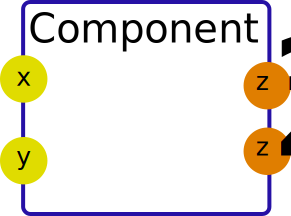
\includegraphics[width=1.1\textwidth]{images/component-cartoon}
    \end{column}
    \begin{column}{.55\textwidth}
      \begin{align*}
        execute(x,y) &\longrightarrow z_1, z_2 \\
        list\_deriv\_vars() &\longrightarrow (x,y), (z_1,z_2) \\
        provideJ(x,y) &\longrightarrow 
        \left[\begin{array}{cc}
          \frac{\partial z_1}{\partial x} & \frac{\partial z_1}{\partial y}\\
          \frac{\partial z_2}{\partial x} & \frac{\partial z_2}{\partial y}\\
        \end{array}\right]\\ 
      \end{align*}
    \end{column}
  \end{columns}
}

\frame{
  \frametitle{OpenMDAO computes the multidisciplinary \\
              derivatives automatically}
  \begin{columns}
    \begin{column}{.4\textwidth}
      \includegraphics[width=\textwidth]{images/total_v_partial}
    \end{column}
    \begin{column}{.6\textwidth}
    %Optimizer needs total derivatives ($\frac{df}{dx_1},\frac{df}{dx_2}$)

    Components provide their partial derivatives: 
    \begin{itemize}
       \item C1: $\frac{\partial y_2}{\partial y_1},\frac{\partial y_2}{\partial x_1}$
       \item C2: $\frac{\partial y_1}{\partial y_2}$
       \item C3: $\frac{\partial f}{\partial y_1}, \frac{\partial f}{\partial x_2}$
     \end{itemize}
    \end{column}
  \end{columns}

  \vspace{2.5em}
  \hspace{1.5em}Martins and Hwang's unified derivative equations give $\frac{df}{dx_1},\frac{df}{dx_2}$
  \begin{textblock}{8}(1.2,13.8)\scriptsize
    [Martins and Hwang 2013]
  \end{textblock}
}

\frame{
  \frametitle{Mixed FD/analytic derivatives let you \\
              focus development effort where it will help most}
  \centering
  \includegraphics[width=1.0\textwidth]{images/mixed_derivs_sample_xdsm}
  %annotate with which disciplines have derivatives and which done
}

% \frame{
%   \frametitle{Breaking models down into smaller pieces \\ 
%               makes computing derivatives easier}
%   \centering
%   {\large Small Satellite design model with 7 disciplines}
%   \includegraphics[width=.95\textwidth]{xdsm/cadre_xdsm}

% }

% \frame{
%   \frametitle{Breaking models down into smaller pieces \\ 
%               makes computing derivatives easier}
%   \centering
%   {\large 7 ``disciplines'' are broken down into 39 components}
%   \includegraphics[width=.95\textwidth]{xdsm/cadre_xdsm_large}

% }

\section[Sample Results]{Optimization results from problems with analytic derivatives}
\subsection[Better speed and accuracy]{Improving optimization speed and accuracy}
\tocframe{\tableofcontents[currentsection]}

\frame{
  \frametitle{Aero-structural Wind Turbine Design problem with \\ 
              30 design variables and 105 constraints}
  \centering 
  \includegraphics[width=\textwidth]{images/wt_perspective}

  \begin{textblock}{8}(7,14)\scriptsize
    [Gray, et al.  2014]
  \end{textblock}
}

\frame{
  \frametitle{5x speed up with mixed analytic and FD gradients}
  \centering
  \tiny
  \begin{tabular}{lrr}
      \toprule
                                            & Finite-Difference & Analytic \\
      \midrule
      Objective (COE  in $\cent$/kWh)       & 5.8045  & 5.8042 \\ 
      Max Constraint Violation              & $2.62\times10^{-6}$ & $1.81\times10^{-6}$  \\ 
      \# Major Iterations                   &  143 & 113  \\
      \textcolor{red}{Time Per Major Iteration (minutes)}    &  \textcolor{red}{2.27} & \textcolor{red}{0.59}  \\
      \textbf{Total Run Time (hours)}       &  \textbf{5.43} & \textbf{1.11} \\

      \bottomrule
  \end{tabular}

  \includegraphics[height=.6\textheight]{images/wt_opt_progress_annotated}
}

% \frame{
%   \frametitle{\textbf{Future Work}: Use Analytic derivatives to\\
%               optimize meanline turbomachinery models}
%   %\includegraphics[width=\textwidth]{images/v5_eff_present}
   

%   \begin{columns}
%     \begin{column}{.4\textwidth}
%       \includegraphics[width=\textwidth]{images/incidenceRange}
%     \end{column}
%     \begin{column}{.6\textwidth}
%       %\includegraphics[width=\textwidth]{images/otac_fd_check}
%       \includegraphics[width=\textwidth]{images/incidence_pres}
%       %\includegraphics[width=\textwidth]{images/incidence_pres}
%     \end{column}
%   \end{columns}

% }

% \frame{
%   \frametitle{Accurate derivatives will yield a better optimum}
%   \centering
%   \includegraphics[width=.75\textwidth]{images/otac_fd_check}

% }



\subsection[1000s of design variables]{Conceptual design problems with 1000s of variables}
%\tocframe{\tableofcontents[currentsection]}

\frame{
  \frametitle{Cubesat Mission Optimization with \\
              has 25,292 design vars. and scalable discretization}
  \begin{columns}
    \begin{column}{.4\textwidth}
      \includegraphics[width=\textwidth]{images/cadre_drawing}
    \end{column}
    \begin{column}{.4\textwidth}
      \includegraphics[width=.8\textwidth]{images/allpts_gearth_mcmurdo}
    \end{column}
  \end{columns}

  \begin{textblock}{8}(2,8.5)\scriptsize
    [Hwang, et al.  2014]
  \end{textblock}

  \vspace{1em}
  \centering
  \scriptsize
  \begin{tabular}{r l l l}
      \toprule
      & Variable/Function &  Quantity \\
      \midrule
      maximize             & Data downloaded & 1\\
      \\
      with respect to & B-spline control schedules  & 25200\\
                      & physical design vars. & 92\\
                      \\
      subject to          & charge, current, temp battery constraints & $30$ \\
      \bottomrule
  \end{tabular}
}

\frame{
  \frametitle{OpenMDAO scaled efficiently 1.7e7 variables}
  \centering
  % \begin{tabular}{r l l l}
  %     \toprule
  %     & Variable/Function & Description & Quantity \\
  %     \midrule
  %     maximize            &  & Data downloaded & 1\\
  %     with respect to & B-spline control points  & time varying schedules & 25200\\
  %                     & Solar Panel, Antenna, and Fin & physical design vars. & 92\\
  %                             & & \textcolor{red}{Total} & \textcolor{red}{$25292$} \\
  %     subject to          & charge, current, temp limits  & physical battery constraints & $30$ \\
  %     \bottomrule
  % \end{tabular}


  %\includegraphics[height=.5\textheight]{images/allpts_gearth_mcmurdo}
  %\includegraphics[height=.5\textheight]{images/cadre_opt_progress}\hspace{2em}
  \includegraphics[height=.75\textheight]{images/cadre_var_scaling}

}

\frame{
  \frametitle{Scaling up to 1e7 variables is key for \\ 
              integration with CFD and FEA}
  \centering
  %\includegraphics[width=.7\textwidth]{images/truss_braced}
  \includegraphics[width=.9\textwidth]{images/high-fi-examples}
  %todo: get picture from opencsm, from chris for nozzle geometry

  \begin{textblock}{8}(-.9,5)\scriptsize
    [Hwang, Kenway, \\ Martins  2014]
  \end{textblock}

  \begin{textblock}{8}(7.5,13.5)\scriptsize
    [Heath, et al.  2015]
  \end{textblock}
}


\subsection[MDAO for ``single disciplines'']{An MDAO perspective for ``single disciplinary'' problems  }
%\tocframe{\tableofcontents[currentsection]}


\frame{
  \frametitle{PyMission optimizes a continuous trajectory \\
              with adjoint analytic derivatives}

  \centering
  \hspace{3em}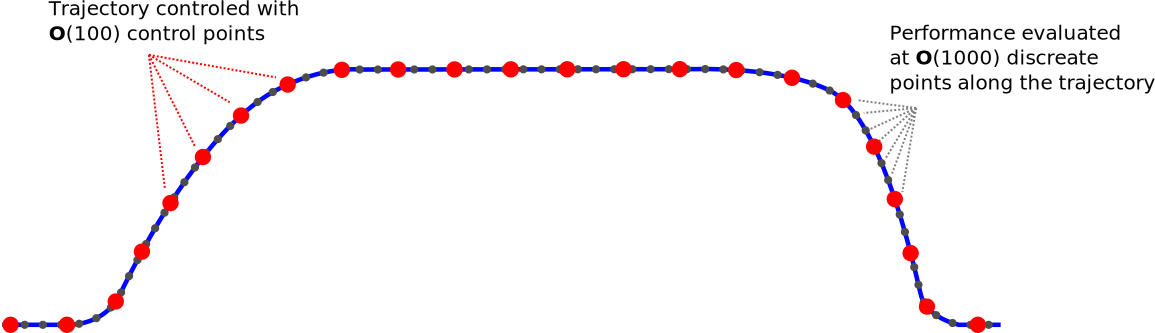
\includegraphics[width=.75\textwidth]{images/pymission_trajectory_cartoon}

  \vspace{1em}
  % \includegraphics[height=.4\textheight]{images/SciTech_CarpetRange_small}
  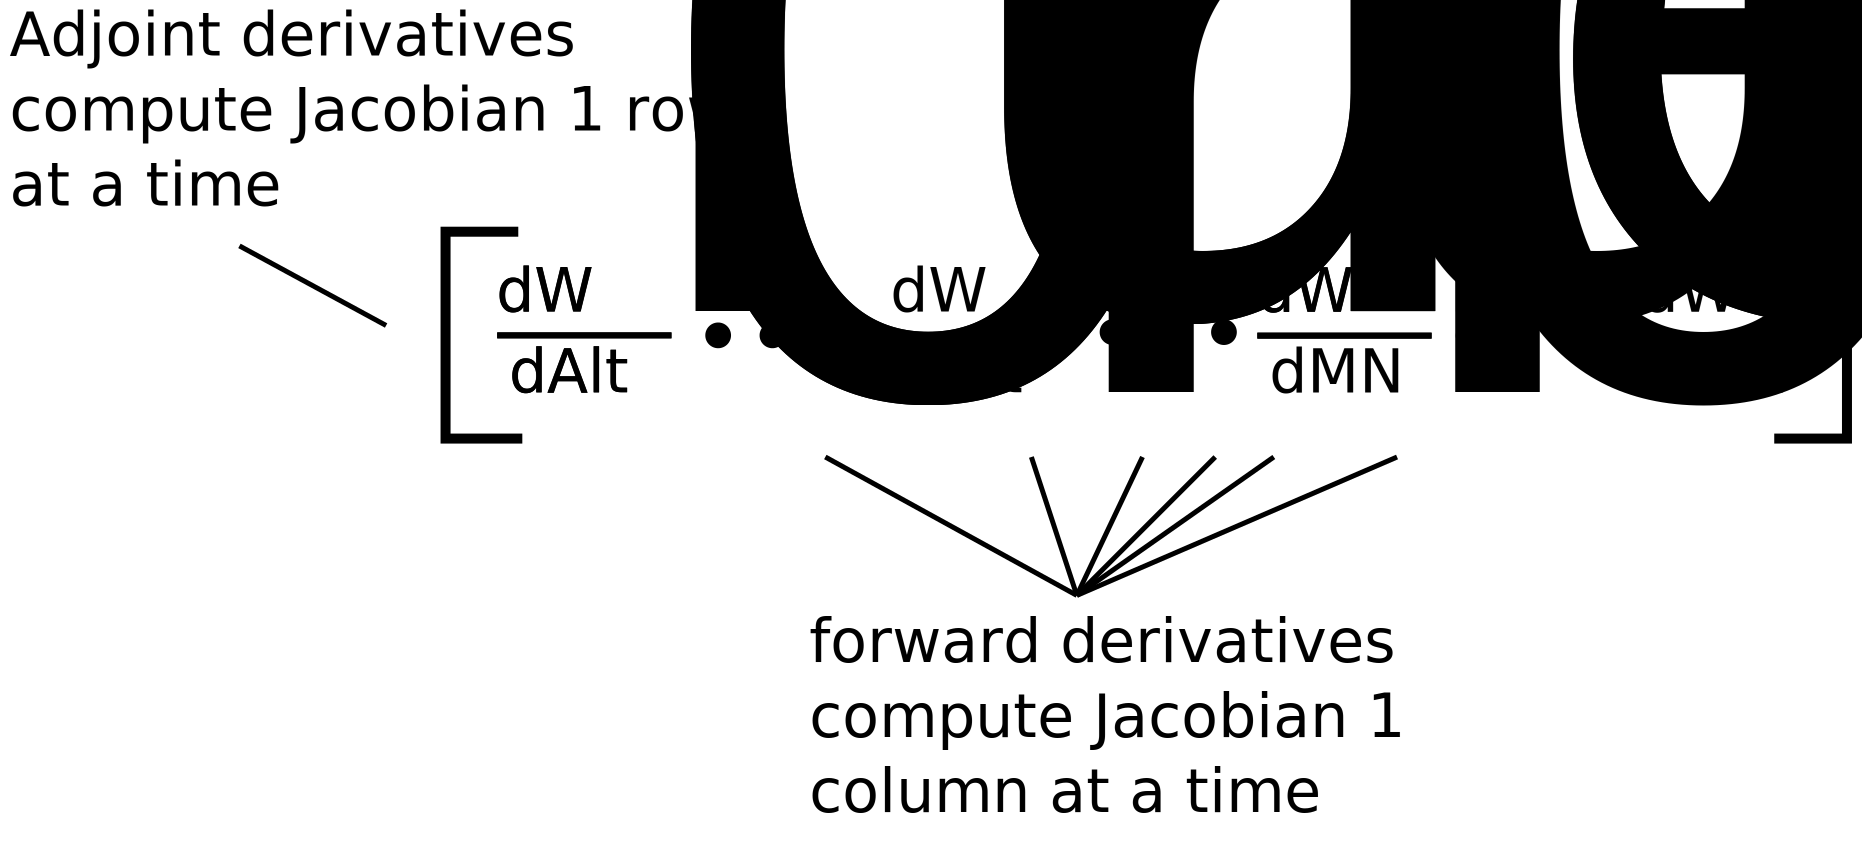
\includegraphics[height=.4\textheight]{images/pymission_jacobian}

  \begin{textblock}{8}(0,13.5)\scriptsize
    [Kao, et al.  2015]
  \end{textblock}
}

\frame{
  \frametitle{Mission analysis is split into sub-disciplines \\
              using OpenMDAO to compute $\frac{d W_{fuel}}{d \txt{alt}}$ and 
              $\frac{d W_{fuel}}{d \txt{MN}}$ }
  \centering
  \includegraphics[width=.9\textwidth]{images/pymission_xdsm}
}

\section[New problems]{Applying OpenMDAO to new problems}
\tocframe{\tableofcontents[currentsection]}

\frame{
  \frametitle{\textbf{Future Work}: nozzle shape optimization \\ 
              couples FUN3D and NPSS}
  \centering
  \includegraphics[width=.75\textwidth]{images/fancy_nozzle_annotated}
}

\frame{
  \frametitle{\textbf{Future Work}: sizing hybrid electric propulsion systems  }
  \centering
  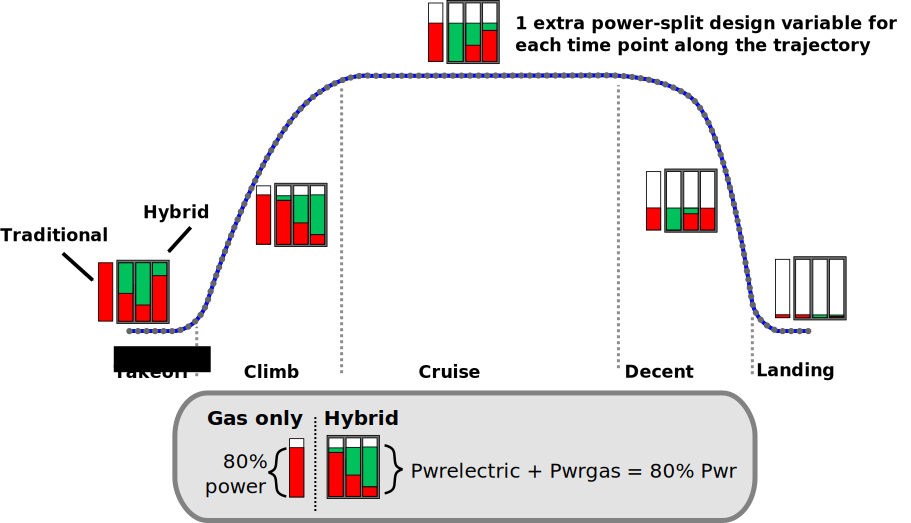
\includegraphics[width=.95\textwidth]{images/trajectory}
}

\frame{
  \frametitle{OpenMDAO provides tools to approach \\
              design problems in new ways }
  \begin{itemize}[itemsep=1em]
    \item Mixed FD/analytic derivatives for better speed and accuracy
    \item Break up single disciplines into sub models \\ to compute 
    derivatives more easily
    \item Adjoint derivatives for problems with high fidelity tools \\ and very large design 
    spaces
  \end{itemize}
}

% \frame{
%   \frametitle{Other problems where analytic derivatives could be useful}
%   \begin{itemize}[leftmargin=.2\textwidth, itemsep=1em]
%     \item Coupled acoustic-CFD for aircraft \\ noise constraints
%     \item Flutter constraints for high AR wings
%     \item Long endurance human powered vehicle \\ with ultra flexible wings
%     \item Optimize ticket cost for Musk's \\ Hyperloop Concept
%   \end{itemize}

% }



\section*{Conclusions}

% {\setbeamertemplate{footline}{} 

%   \frame{
%     \frametitle{OpenMDAO provides a number of ways simplify 
%                 implementation of analytic derivatives}
%     \begin{itemize}[itemsep=1em]
%       \item Break up single disciplines into sub models \\ to compute 
%       derivatives more easily
%       \item Adjoint derivatives for problems with 1000s of design variables
%       \item Mixed FD/analytic derivatives for better speed and accuracy
%     \end{itemize}
%   }
% }

{ \setbeamertemplate{footline}{}  
  \frame{ 
    \frametitle{Acknowledgments}

      \begin{textblock}{4.5}[.5,.5](8,4)
        \includegraphics[width=.9\textwidth]{images/NASA_logo}
      \end{textblock}

    \vspace{5em}
    \begin{itemize}[itemsep=1em]
      \item TAC Transformational Tools and Technologies Project
      \item Dr. Joaquim Martins, Dr. John Hwang, and Jason Kao from University of Michigan
      \item Dr. Andrew Ning and Katherine Dykes from National Renewable Energy Laboratory
      \item Christopher Heath and Eric Hendricks from the NASA Glenn Research Center
    \end{itemize}

      % \begin{textblock}{8}(.5,12.5)
      %   \includegraphics[width=\textwidth]{images/Umich_Aero_logo_horiz}
      % \end{textblock}

      % \begin{textblock}{5}(10,12.8)
      %   \includegraphics[width=\textwidth]{images/nrel-logo}
      % \end{textblock}

      \begin{textblock}{12}(3.5,14)
        
\includegraphics[width=.75\textwidth]{images/openmdao-logo}
      \end{textblock}
  }
}


%These are just a few examples of of design problems with a 
%mixture of different fidelities and very large design spaces. 
%The new features in OpenMDAO make it much easier to integrate analytic derivatives 
%into system models and use them to solve more complex design problems. 

\end{document}